\documentclass{standalone}
\usepackage{tikz}
\usepackage{ctex,siunitx}
\setCJKmainfont{Noto Serif CJK SC}
\usepackage{tkz-euclide}
\usepackage{amsmath,mhchem}
\usetikzlibrary{patterns, calc}
\usetikzlibrary {decorations.pathmorphing, decorations.pathreplacing, decorations.shapes,}
\begin{document}
\small
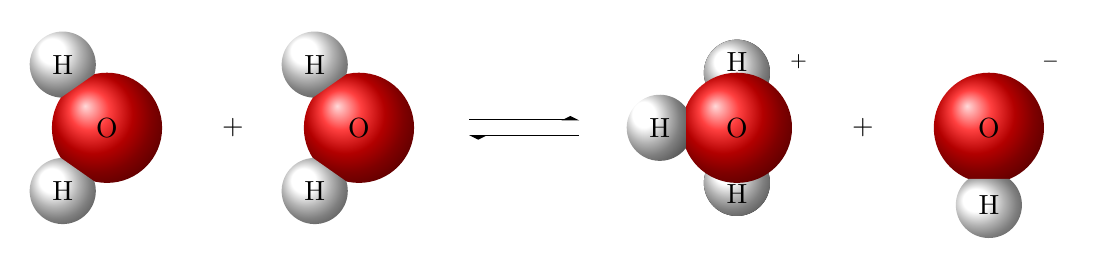
\begin{tikzpicture}[>={Diamond[left]},scale=2.0]
  \begin{scope}[scale=0.7]
    \tkzDefPoints{0/0/O,0/0.5/R}
    \tkzDefPoint(125:0.7){H1}
    \tkzDefPoint(125:1){r1}
    \tkzDefPoint(235:0.7){H2}
    \tkzDefPoint(235:1){r2}
    \tkzInterCC(O,R)(H1,r1)\tkzGetPoints{A}{B}
    \tkzInterCC(O,R)(H2,r2)\tkzGetPoints{C}{D}
    \tkzDrawCircle[draw=none,ball color=red](O,R)
    \tkzDrawArc[draw=none,ball color=white](H1,B)(A)
    \tkzDrawArc[draw=none,ball color=white](H2,D)(C)
    \node at (O) {\ce{O}};
    \node at (H1) {\ce{H}};
    \node at (H2) {\ce{H}};
  \end{scope}
  \node at (0.8,0){\normalsize $+$};
  \node at (4.8,0){\normalsize $+$};
  \draw[->](2.3,0.05)--++(0.7,0);
  \draw[<-](2.3,-0.05)--++(0.7,0);
  \begin{scope}[xshift=1.6cm,scale=0.7]
    \tkzDefPoints{0/0/O,0/0.5/R}
    \tkzDefPoint(125:0.7){H1}
    \tkzDefPoint(125:1){r1}
    \tkzDefPoint(235:0.7){H2}
    \tkzDefPoint(235:1){r2}
    \tkzInterCC(O,R)(H1,r1)\tkzGetPoints{A}{B}
    \tkzInterCC(O,R)(H2,r2)\tkzGetPoints{C}{D}
    \tkzDrawCircle[draw=none,ball color=red](O,R)
    \tkzDrawArc[draw=none,ball color=white](H1,B)(A)
    \tkzDrawArc[draw=none,ball color=white](H2,D)(C)
    \node at (O) {\ce{O}};
    \node at (H1) {\ce{H}};
    \node at (H2) {\ce{H}};
  \end{scope}
  \begin{scope}[xshift=4.0cm,scale=0.7]
    \tkzDefPoints{0/0/O,0/0.5/R,-0.7/0/H1,-1/0/r1}
    \tkzInterCC(O,R)(H1,r1)\tkzGetPoints{A}{B}
    \fill[ball color=white](0,0.5)circle(0.3);
    \fill[ball color=white](0,-0.5)circle(0.3);
    \tkzDrawCircle[draw=none,ball color=red](O,R)
    \tkzDrawArc[draw=none,ball color=white](H1,B)(A)
    \node at (45:0.8){$^+$};
    \node at (O) {\ce{O}};
    \node at (H1) {\ce{H}};
    \node at (0,0.6) {\ce{H}};
    \node at (0,-0.6) {\ce{H}};
  \end{scope}
  \begin{scope}[xshift=5.6cm,scale=0.7]
    \tkzDefPoints{0/0/O,0/0.5/R,0/-0.7/H1,0/-1/r1}
    \tkzInterCC(O,R)(H1,r1)\tkzGetPoints{A}{B}
    \tkzDrawCircle[draw=none,ball color=red](O,R)
    \tkzDrawArc[draw=none,ball color=white](H1,B)(A)
    \node at (45:0.8){$^-$};
    \node at (O) {\ce{O}};
    \node at (H1) {\ce{H}};
  \end{scope}
\end{tikzpicture}
\end{document}